% PACKAGES INCLUDED HERE 
% DO NOT NEED TO CHANGE
\documentclass[conference]{IEEEtran}
%\IEEEoverridecommandlockouts
% The preceding line is only needed to identify funding in the first footnote. If that is unneeded, please comment it out.
\usepackage{cite}
\usepackage{amsmath,amssymb,amsfonts}
\usepackage{algorithmic}
\usepackage{graphicx}
\usepackage{textcomp}
\usepackage{multicol}
\def\BibTeX{{\rm B\kern-.05em{\sc i\kern-.025em b}\kern-.08em
    T\kern-.1667em\lower.7ex\hbox{E}\kern-.125emX}}
\begin{document}

% TITLE GOES HERE

\title{Utilizing Q-Learning Variations to Play \textit{Galaga}\\}
% AUTHOR NAMES GOES HERE

\author{\IEEEauthorblockN{Nathan Byrnes}
\IEEEauthorblockA{\textit{Computer Science} \\
\textit{Middle Tennessee State University}\\
Murfreesboro, USA \\
ndb3w@mtmail.mtsu.edu}
\and
\IEEEauthorblockN{Christopher Gerspacher}
\IEEEauthorblockA{\textit{Computer Science} \\
\textit{Middle Tennessee State University}\\
Murfreesboro, USA \\
cag7a@mtmail.mtsu.edu}
\and
\IEEEauthorblockN{Jonathan Gregory}
\IEEEauthorblockA{\textit{Computer Science} \\
\textit{Middle Tennessee State University}\\
Murfreesboro, USA \\
jbg4a@mtmail.mtsu.edu}
\and
\IEEEauthorblockN{Cameron Justice}
\IEEEauthorblockA{\textit{Computer Science} \\
\textit{Middle Tennessee State University}\\
Knoxville, USA \\
cj4g@mtmail.mtsu.edu}
\and
\IEEEauthorblockN{Ian Seal}
\IEEEauthorblockA{\textit{Computer Science} \\
\textit{Middle Tennessee State University}\\
Murfreesboro, USA \\
ins2c@mtmail.mtsu.edu}
\and
\IEEEauthorblockN{Justin Wade}
\IEEEauthorblockA{\textit{Computer Science} \\
\textit{Middle Tennessee State University}\\
Murfreesboro, USA \\
jww5f@mtmail.mtsu.edu}
}

\maketitle

% ABSTRACT 

\begin{abstract}

The Deep Q-Learning architecture and its advancements allow for human-level learning of retro games. However, it is rare for any Deep Q-Learning studies to cover the 1981 classic arcade game \textit{Galaga}. Building off Double Q-Learning and Prioritized Experience Replay advancements, we compared four stable Deep Q-Learning models over 1000 epochs to compare their ability to learn Galaga in short-term training. We have concluded that in short-term training sessions, the Single-Q Prioritized network is the most applicable, but given further training time we believe that the Double-Q Prioritized network would be the most applicable for \textit{Galaga}.
\end{abstract}

% KEYWORDS
\begin{keywords}
\textit{Keywords}: Neural Network, Q-Learning, Replay Memory, Galaga
\end{keywords}

% INTRODUCTION SECTION
\section{Introduction}

Since 1981, \textit{Galaga} has been a classic arcade title and a popular favorite for many. On the surface, \textit{Galaga} is a simple game with the singular goal being to score the highest point total possible. However, the challenge of \textit{Galaga} comes from difficulty introduced via the speed increases of the game and the increasingly complex movement patterns as the levels increase. It is because of these factors that we decided \textit{Galaga} is the perfect candidate for various implementations of deep Q-learning networks and see how well these networks succeed at getting the highest score. The Q-learning networks we decided on are: Single Q with Uniform Replay Memory, Single Q with Prioritized Replay Memory, Double Q with Uniform Replay Memory, and Double Q with Prioritized Replay Memory. By utilizing multiple implementations, we can better understand how these networks are both similar and different from each other; mainly, both in how they learn and in how they tune themselves to perform more efficiently. \par
Our goal in this project was to use the results of these implementations to compare and contrast the performance of each network based on score within the game, with the final goal to mimic human game play or surpass it entirely. Therefore, finding the best implementation of this can display how well the combination of neural network methodology mimics that of human experience and learning. \par
Our initial hypothesis was that the Single-Q Prioritized model would show the most prominent rate of learning, but that the Double-Q Prioritized would show the greatest improvement. Further, the Uniform implementations would show the worst performance, but share a common trend in learning. 

% BACKGROUND SECTION
\section{Background}

Numerous studies have been done on deep reinforcement learning and its variations, with each study and improvement including a comparison of performance, commonly across Atari games. Beginning with the original Deep Q-Learning \cite{Mnih2015} adaptation of algorithmic Q-Learning\cite{Watkins1989}, what we refer to as "Single Q-Learning Uniform Experience Replay", these games neglected to include the 1981 hit-classic, \textit{Galaga}. \par
Further advancements upon Deep Q-Learning that we used, \textit{Prioritized Experience Replay}\cite{schaul2015prioritized} and \textit{Deep Reinforcement Learning with Double Q-Learning} \cite{hasselt2015deep}, also neglected to cover \textit{Galaga}, and failed to compare the prioritized experience replay implementation within single and double q-learning implementations. \par
Q-Learning networks learn the Q function, a function of state-action pair inputs, $Q(S,A)$, in regular Q-Learning, but defined as a function of state, $Q(S)$, within Deep Q-Learning, producing an array of Q values respondent to each action, declaring the highest given Q value as the action to input. The network model is guided by $Q_{target}$, acting as the best it can do, and focusing progress. \par
The addition of the replay memory allowed Deep Q-Learning to remove its biases and data issues and be usable and provable \cite{Mnih2015}. The addition of Double Q-Learning allowed for a reduction of overestimation in the network's action evaluation \cite{hasselt2015deep}. Finally, Prioritized Experience Replay allowed for a more focused replay of experiences, leading to a faster learning rate for networks by keeping experiences that could be more useful \cite{schaul2015prioritized}. \par
Our interest in these methods within \textit{Galaga} was peaked by a small excursion we had into implementing the basic DQN agent to play Kirby's Adventure (Nintendo, 1993), which we determined to be a much more complex task than many areas covered in previous studies. With only the basic implementation, we saw evidence of learning after about 25 million frames experienced. As this was an intensive task computationally, we believed that the best place to experiment with further DQN implementations would be in a smaller action space, and as \textit{Galaga} had not been covered, we determined this to be an excellent context for research. \par
Methods used in past studies covered how to convey progress to the network, the primary methods being Reward Normalization and Negative Stabilization. Reward Normalization attempts to clamp game rewards that are too large in order to more accurately portray performance to the network. Negative Stabilization attempts to punish the agent when its experience leads it to a plateau, such as a point where it lives as long as possible, but does so by not increasing its score. \par
Multiple studies done in the past have determined that gray-scaling the image of the scene allows for a reduced network size, faster processing, and ultimately a faster training time than keeping the image in full color. As this is solidified in research, we decided to implement this as well.
By implementing each of these methods, we hope to determine the best implementation of Deep Q-Learning within the \textit{Galaga} context, and to reaffirm prior research into the best implementation for the greater Reinforcement Learning context.

% METHODS SECTION
\section{Methods}
The Q-Learning mechanism \cite{Watkins1989}, utilized a policy-iteration technique around potential rewards to develop the correct response action for a given scenario. The Deep Q-Learning architecture \cite{Mnih2015}, is an extension of the Q-Learning mechanism and utilizes a neural network to approximate the Q-value function and requires replay memory in order to train properly. For the initial \textit{Galaga} network we used Deep Q-Learning and Single Q-Learning Uniform replay memory. From the initial network, we were able to compare with five other architectures: Random, Deep Q-Learning with Uniform replay memory, Deep Q-Learning with Prioritized memory replay, Double Q-Learning with Uniform replay memory, and Double Q-Learning with Prioritized memory replay.  \par
We utilized both Prioritized and Uniform replay memory in order to obtain an analysis on the efficiency of different network structures. Uniform replay memory is simply experience replay without prioritization. Experience replay allows our network to learn through an agent that memorizes and reuses past experiences.  Prioritized replay memory allows us to prioritize the experience by its temporal difference error, $Q{target} - Q$. However, sampling purely based on TD error introduces a bias to the network learning \cite{schaul2015prioritized}. To treat this, we used importance sampling weights for bias correction. \par
Our networks were built using the tools provided by the Tensorflow and Tensorflow Keras python libraries. Our input data was provided by the OpenAI Retro Gym, and includes full per-pixel data of the screen after an action is taken. The input data consists of a by-pixel image after the last action is executed. The image is of height 84px, width 84px, and is gray scaled to exhibit only one value per pixel, resulting in an input size of 7,056. Our output data data consists of a vector mapping to one of five actions in the Action Space, as a one dimensional vector of \textit{Galaga}'s actions: Move Left, Move Right, Fire, and combinations of moving and firing. The OpenAI Retro Gym allows us to have a view-less, increased speed version of the game, which can speed up training times.\par
The network architecture consists of a sequential model following a similar architecture used in previous Deep Q-Learning papers, with convolution layers of 64, 32, and 16, with a pooling layer after the first and last. From there we flatten before passing through two dense layers of size 1024 and 512, with an output layer of 15 matching the action size of \textit{Galaga}. That provides us the trainable parameters which get updated during backpropagation. The first convolution layer (Conv2D) has 64 feature detector units that we slide around the image. Each feature detector makes a kernel size of 7 x 7, and the keras framework automatically sets up the layer to slide each of the feature detectors across all 7 x 7 regions in the image. The second convolution layer has 32 feature detector units and a kernel size of 5 x 5, and the third convolution layer has 16 feature detectors which also uses a 5 x 5 kernel size. The rectified linear activation function (ReLU) is utilized by both our convolution layers and dense layers, while the softmax activation function is utilized by the output layer.\par
Before training, each network was initialized with a weight set generated under the same seed to ensure comparability. At each state, represented by the current frame of the game, the network receives the frame and generates Q-values, the highest of which designating the action to execute. Once the action is executed, we observe the reward and the next state, and store the experience in the replay memory bank. This is repeated over a course of 1,000 epochs(episodes), limiting each epoch to a maximum of 20,000 experiences, and over time accumulate experiences within the replay memory bank. The more episodes that progress the more control the net gains by reducing the epsilon, thereby reducing the chance of random action. By forcing the net at to experience random actions it will explore more actions that could increase reward, and allow it to generate a better policy. The more that the network experiences, the more it has learned, and can choose the proper action more often. Once it is complete we evaluate it and compare to previous runs in order to find the most optimized hyper parameters and architecture. Each model was trained and evaluated under the same hyper-parameters and limits, which allows for a direct comparison of all models. Each fit of the model covers one play through of the game, beginning at the first level and continuing until the unit is out of lives or has completed the final level.\par
To complement our agents, we implemented Negative Stabilization and Reward Normalization equally for each agents. For negative stabilization, we introduced a negative reward of 10 points if the agent went 50 frames without experiencing a change in score. For reward normalization, we clamped the unit scores between [-10,1] as without this, the agent could experience a maximum reward of 3000, but with an average reward of 400. Leaving the reward this way would result in certain rare experiences being more important, and the average experience being less useful to training. By clamping the reward value, we make all experiences separable to either an increase in score, or a plateau.

% RESULTS SECTION
\section{Results}
After training each model for 1000 epochs, we graphed their mean score following each epoch to track their progress. Figures (1-4) (shown at end) display the mean score progression for the models. Because a drastic change in mean score is more difficult as time progresses, trends are more noticeable in this method of analysis. For comparison, we also ran a completely random agent, based on the same seed, across 1000 epochs, and displayed its progress in Figure (5). Further, as a simple extra data point, we had one team member play 20 games, and recorded his mean score at 29,651. \par
Our annealing schedule placed an absolute epsilon minimum (set at 0.01) to be reached at the 457th epoch. The network has primary control (epsilon=0.5) at the 68th epoch. All graphs show a similar sign of control around 100th-160th epochs (epsilon=0.36, 0.19).
As we expected, the prioritized replay models showed a much faster rate of change, with both the Single-Q and Double-Q showing an upward trend past the 600th epoch. Comparatively, the uniform replay models showed no definitive trend by the end of the training session, and presented a much smaller rate of change across the session. \par
Visually, each of the agents developed basically the same strategy, which is sitting in the middle of the screen and firing for the majority of the time. The agent would move from that position only when units are lacking, or to avoid enemy attacks. However, the Single-Q Prioritized agent showed the most movement from its center position, leading us to believe that the agents ended within a "dead-zone" of sorts, where they have begun maximizing their ability to increase their score over time, but have not yet experienced enough epochs where their score trend did not increase.

% DISCUSSION SECTION
\section{Discussion}
Our initial hypothesis was proven incorrect, and in fact Double-Q Prioritized exhibited the highest rate of learning and the greatest increase in performance. However, Single-Q Prioritized exhibited the highest level of performance at the end of the session, leading us to believe that the overestimation caused by Single Q-Learning could be a benefit to short-term learning if optimizing only for total performance. This agent's difference in visual behavior could be further evidence for it being the fastest learning agent. \par
The Uniform agents showed the worst performance change, with Single-Q Uniform being in a downward slope at the end of its session, and experiencing a very slight upward trend across its full-control (post 457th epoch) section of the session. Double-Q Uniform was on a plateau at the end of its session, and showed a very negative trend across its full-control section of the session. \par
For posterity, we recognize that compared to our 20-Epoch human average and our random agent, all four models failed to surpass them, and we attribute this to the high number of experiences that must occur before a network can properly learn. \par
As per our goal, we believe that, in short-term learning sessions, Single-Q Prioritized agents will show the greatest performance, but Double-Q Prioritized will show the most learning. As per our results, Single-Q implementations are not recommended for short-term learning sessions.
Further research in this area would require longer training sessions, matching those of the previous studies that reach 200 million experiences (compared to our \texttildelow 5 million experiences). We believe these small training sessions are the primary fault in our research, but our computing ability limited our available training time. \par
We would also implement Frame Skipping, which batches frames to more properly model human learning, and reduces overall network passes while keeping the total number of experiences. This would have advanced our frames experienced to roughly 20 million, and could have allowed for longer training sessions.\par

\section{Conclusion}
In this research we have implemented the Deep Q-Learning Neural Networks architecture within four variations: Single Q-Learning Uniform Experience Replay, Single Q-Learning Prioritized Experience Replay, Double Q-Learning Uniform Experience Replay, and Double Q-Learning Prioritized Experience Replay. We have run each of these for 1000 epochs under the same parameters to conclude which method is the best used to play the 1981 arcade classic, \textit{Galaga}. Through this, we have concluded that in short-term training sessions the Single-Q Prioritized network is the most applicable, but given further training time we believe that Double-Q Prioritized would be the most applicable for \textit{Galaga}.

% REFERENCES
% THIS IS CREATED AUTOMATICALLY
\bibliographystyle{IEEEtran}
\bibliography{References} % change if another name is used for 
\clearpage

\onecolumn
\section*{\centering{Figures}}

\begin{figure}[h]
\centering
\begin{minipage}{.5\textwidth}
     \centering
    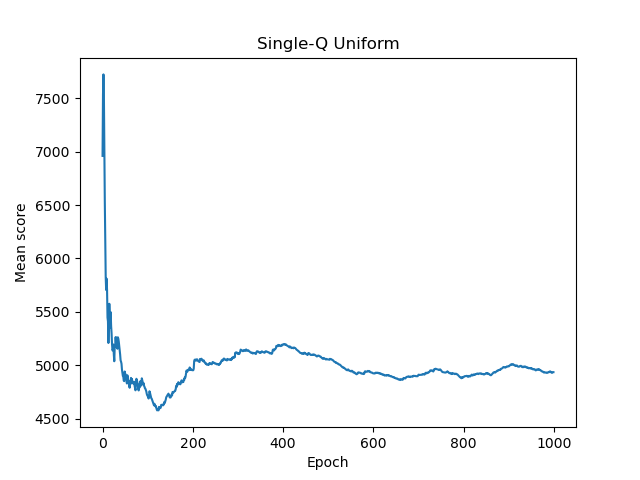
\includegraphics[width=.91\textwidth]{SQU.png}
    \caption{Mean Score of Single-Q Uniform}
\end{minipage}%
\begin{minipage}{.5\textwidth}
     \centering
    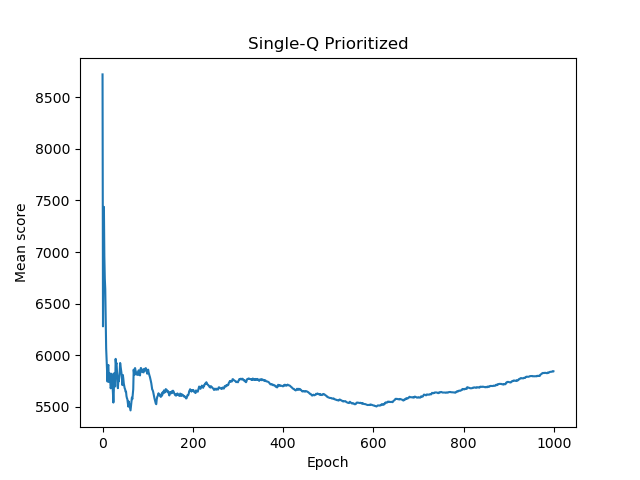
\includegraphics[width=.91\textwidth]{SQP.png}
    \caption{Mean Score of Single-Q Prioritized}
\end{minipage}

\centering
\begin{minipage}{.5\textwidth}
     \centering
    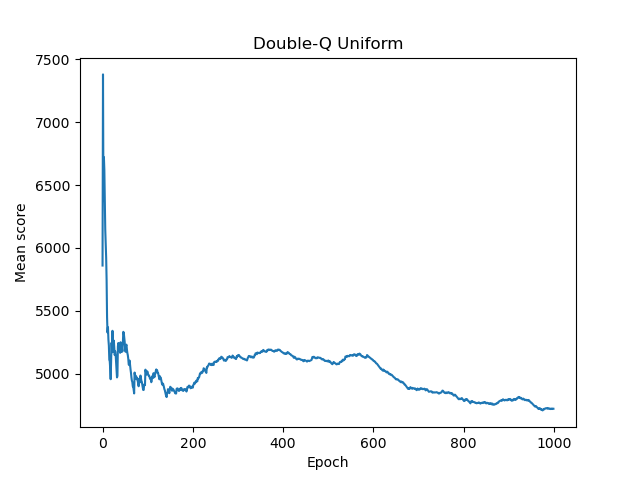
\includegraphics[width=.91\textwidth]{DQU.png}
    \caption{Mean Score of Double-Q Uniform}
\end{minipage}%
\begin{minipage}{.5\textwidth}
     \centering
    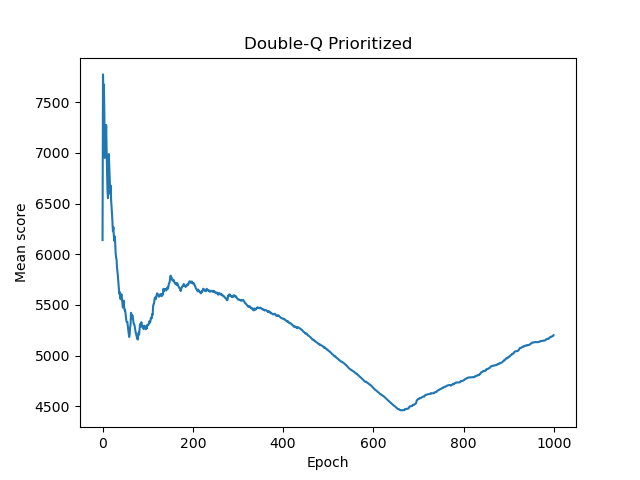
\includegraphics[width=.91\textwidth]{DQP.png}
    \caption{Mean Score of Single-Q Prioritized}
\end{minipage}

\centering
\begin{minipage}{.5\textwidth}
    \centering
    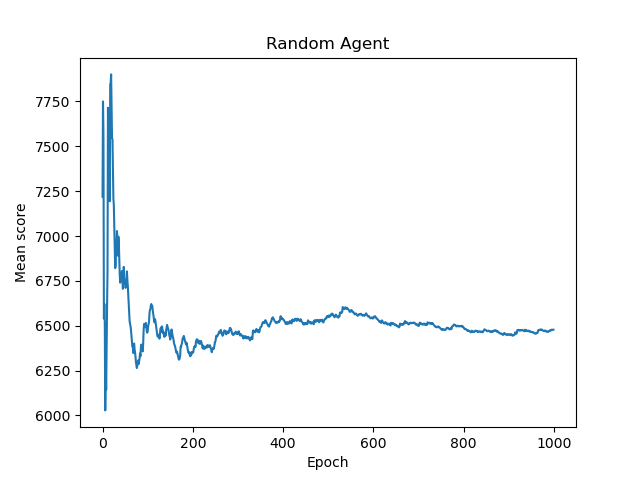
\includegraphics[width=.91\textwidth]{rand.png}
    \caption{Mean Score of Random Agent}
\end{minipage}%
\end{figure}

\end{document}
